\chapter{Propriétés d'un désordre de type speckle}
\label{ch:Speckle}
%\begin{tikzpicture}[remember picture, overlay]
%\node[anchor=north east,inner sep=0pt] at (current page.north east) {
\includegraphics[scale=1]{Fig/Speckle/g825.png}};
%\end{tikzpicture}

Le chapitre \ref{ch:BEC_manip} nous a renseigné quant aux propriétés de notre onde de matière ainsi que sa production. En particulier, on a vu qu'il était possible d'appliquer des potentiels externes conservatifs aux atomes par le biais du potentiel dipolaire. Ce potentiel étant proportionnel à l'intensité lumineuse $I$, on peut alors appliquer un désordre à nos atomes, pourvu que l'on soit capable de créer un désordre optique. En effet, une originalité de notre expérience est "d'inverser" les rôles habituels de la matière et de la lumière.

Ainsi, dans ce chapitre, nous allons nous attacher à décrire le second élément clé de la localisation d'Anderson: le désordre. Nous montrerons que la génération d'un tel désordre est aisée: la diffraction d'un faisceau laser au travers d'une lame de verre rugueuse produit un motif d'intensité lumineuse aléatoire et à fort contraste, appelé champs de tavelures optiques, ou encore \emph{Speckle} (anglicisme communément admis). Citons deux énormes avantages d'un tel désordre: on en connaît toutes les propriétés, régies par la diffraction, et on contrôle ce désordre. 

La première partie se concentrera sur la génération d'un champ de speckle, en particulier sur le diffuseur qui donne au speckle toutes ses propriétés. Dans un second temps, nous décrirons les propriétés spatiales d'un speckle, en particulier la taille des grains de lumière dans les directions transverses et longitudinale. Dans une troisième partie nous parlerons du potentiel ressenti par les atomes ainsi que des possibilités offertes par la structure multi-niveaux du \isotope[87]{Rb} et l'excellent contrôle du désordre dont nous disposons, puis dans une ultime partie nous étudierons une approche à deux longueurs d'onde pour dépasser les limitations d'un speckle monochromatique pour l'étude de la transition d'Anderson à énergie résolue. 

\section{Génération d'un champ de speckle}
%\section{Propriétés statistiques d'un champ de speckle}
C'est avec le développement des premiers lasers qu'a été observée la structure granulaire de la lumière réfléchie par certaines surfaces rugueuses. Rapidement, il a été compris que ce motif provenait de la diffraction aléatoire et cohérente par une surface rugueuse. 
Cette surface rugueuse peut-être considérée comme un ensemble d'émetteurs cohérents de déphasages aléatoires, et le profil d'intensité obtenu est le résultat de l'interférence multiple de l'ensemble de la surface. Un profil typique est montré figure \ref{fig:speckle_pattern}. Celui-ci comporte un ensemble de grains lumineux séparés par des zones d'obscurité.
Souvent considéré néfaste dans le domaine de l'imagerie, le speckle est pour nous une formidable source de désordre optique. 

\begin{figure}
\centering
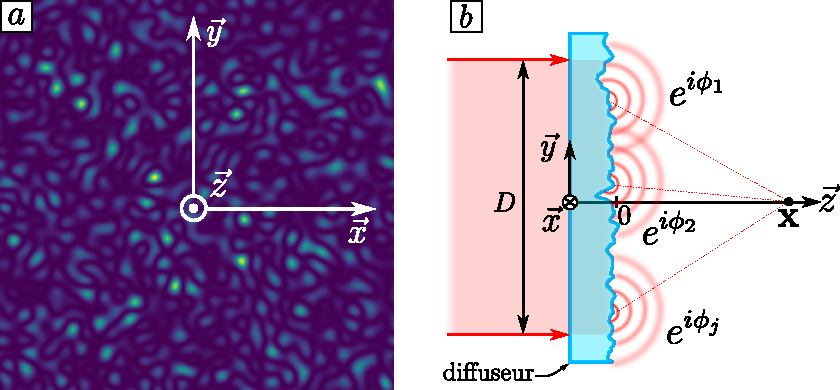
\includegraphics[width=0.9\textwidth]{Fig/Speckle/speckle_pattern.pdf}
\caption{\textbf{a: Motif de speckle.} Un tel motif est composé de grains lumineux entourés de zones d'ombre, où l'intensité est quasiment nulle. \textbf{b: Génération d'une figure de speckle.} La diffraction d'une onde cohérente par une surface rugueuse appelée diffuseur résulte en l'interférence multiple d'une grand nombre d'ondes à déphasage aléatoire. La phase de chacune de ces ondes est déterminée par l'épaisseur de verre traversée en chaque point.}
\label{fig:speckle_pattern}
\end{figure}



\subsection{Statistiques de l'intensité d'un speckle}

Le phénomène de speckle apparaît lorsque l'amplitude $E(\mathbf{x})$ au point d'observation $\mathbf{x}$ résulte de la somme d'un grand nombre N d'ondes indépendantes d'amplitude $E_0$ et de phases aléatoires $\phi_j$ comme illustré figure \ref{fig:speckle_pattern}. Cette amplitude peut alors s'écrire
\begin{equation}
E(\mathbf{x})=\sum_{j}^{N} E_0 e^{i \phi_j} \text{ .}
\end{equation}
En supposant qu'un grand nombre de grains du diffuseur participent à l'interférence au point d'observation ($\rdiff \ll D$ avec $\rdiff$ la taille typique d'un grain du diffuseur et $D$ la taille de l'éclairement incident), on peut appliquer le théorème central limite à l'amplitude rayonnée. En supposant de plus que les phases aléatoires $\phi_j$ sont réparties de manière homogène sur l'intervalle $\left[ 0,2\pi \right]$, les distributions de probabilités des parties réelle et imaginaire de l'amplitude sont données par la loi normale
\begin{equation}
\mathcal{P}(E_{\mathcal{R,I}})=\frac{1}{\sigma_E\sqrt{2\pi}} \exp{\left( -\frac{E_{\mathcal{R,I}}^2}{2 \sigma_E^2}\right) } \text{ ,}
\end{equation}
avec $E_{\mathcal{R}}$ et $E_{\mathcal{I}}$ les parties réelle et imaginaire du champ complexe $E=E_{\mathcal{R}} +i E_{\mathcal{I}}$ respectivement. Étant donné que les atomes ne sont sensibles qu'à l'intensité lumineuse $I=\left| E \right| ^2$, on montre alors que la distribution de probabilité de l'intensité lumineuse suit une loi exponentielle \citep{goodman2007speckle}
\begin{equation}
\mathcal{P}(I)=\frac{1}{\overline{I}}\exp{\left( -I/\overline{I} \right) } \text{ .}
\label{eq:proba_speckle}
\end{equation}
De manière générale, on appellera \emph{speckle pleinement développé} tout speckle vérifiant cette loi de probabilité. Deux conséquences importantes de cette loi sont à noter:
\begin{itemize}
\item[\textendash] L'écart-type $\sigma_I$ de la loi \ref{eq:proba_speckle} est égal à sa valeur moyenne $\overline{I}$, et donc le contraste $\sigma_I /\overline{I}$ d'une figure de speckle pleinement développé est de 1. Une telle figure comportera alors des zones de forte intensité tout comme des zones d'intensité quasi-nulle. 
\item[\textendash] La probabilité d'obtenir une forte intensité lumineuse est exponentiellement petite, tandis que les zones de faible intensité sont beaucoup plus probables. Ainsi, une figure typique de speckle (représentée figure \ref{fig:speckle_pattern}) est composée de maxima d'intensité lumineuse (\emph{grains de speckle}) entourés de larges zone d'ombre.
\end{itemize}





\subsection{Propriétés du diffuseur}
\label{sc:prop_diffuseur}
L'analyse précédente décrivant la statistique de l'intensité lumineuse d'un speckle pleinement développé repose sur deux hypothèses: 
\begin{itemize}
\item[\textendash] Il faut qu'un grand nombre d'émetteurs participe à l'interférence au point d'observation. Notamment, cela signifie que le diffuseur comporte un nombre suffisamment de \emph{grains} ($\rdiff \ll D$)  et que ceux-ci rayonnent au point d'observation. Ce dernier point sera illustré section \ref{sc:speckle_correlation}.
\item[\textendash] Pour que la distribution de probabilité de l'amplitude soit centrée en 0, propriété essentielle pour un speckle pleinement développé, il faut que la distribution de phases soit suffisamment large, c'est à dire $\sigma_\phi \gg 2\pi$. 
\end{itemize}
Les deux grandeurs apparaissant dans ces hypothèses, $\rdiff$ et $\sigma_\phi$, sont fixées par les propriétés du diffuseur, que nous nous attacherons à décrire dans cette partie.

Dans le cadre de notre expérience, la génération du speckle se fait par transmission d'une onde laser au travers d'une lame de verre dépolie, d'épaisseur locale $e(\mathbf{x}_0)$ aléatoire et répartie selon une distribution gaussienne de largeur $\sigmae$ et de valeur moyenne $\overline{e}$, où $\overline{\:\cdots\:}$ représente la moyenne sur les différentes réalisations de l'épaisseur aléatoire. On supposera que cette lame a été dépolie de manière homogène, ainsi, la statistique de l'épaisseur ne dépend pas de la position considérée sur la surface du diffuseur. On assimilera donc la distribution de l'épaisseur à un processus stationnaire. 

La phase localement accumulée par le faisceau laser incident lors de la traversée du diffuseur est proportionnelle à l'épaisseur traversée et donnée par
\begin{equation}
\phi(\mathbf{x}_0)=2\pi (n-1) \frac{e(\mathbf{x}_0)}{\lambda} \text{ ,}
\end{equation}
avec $n$ l'indice du verre et $\lambda\approx \SI{780}{\nano\metre}$ la longueur d'onde de l'onde laser. L'influence de cette phase sur l'amplitude du champ laser se traduit via la transmission locale du diffuseur
\begin{equation}
\tdiff(\mathbf{x}_0)=e^{i\phi(\mathbf{x}_0)}
\end{equation}
dont la valeur moyenne $\overline{\tdiff}$ caractérise le pouvoir diffusant. Pour une lame peu rugueuse, le faisceau est en moyenne peu affecté lors de sa traversée et l'on a $\overline{\tdiff}\approx 1$, tandis que dans le cas d'un diffuseur fort $\overline{\tdiff} \approx 0$. En fixant la phase moyenne $\overline{\phi}=0$, on montre annexe \ref{ch:anex_speckle} que \citep{denechaud2018vers}
\begin{equation}
\overline{\tdiff}=e^{-\frac{\sigma_{\phi}^2}{2}} \quad \text{avec} \quad \sigma_\phi=2\pi (n-1) \frac{\sigmae}{\lambda} \text{ .}
\end{equation}
Dans le cas d'un diffuseur de grande rugosité, dont l'épaisseur typique des grains $\sigmae$ est de l'ordre de plusieurs $\lambda$, on a $\sigma_\phi \gg 2\pi$ et cela permet donc de considérer que la distribution de phases est constante sur l'intervalle $\left[0,2\pi \right]$, essentiel pour un speckle pleinement développé.

\begin{figure}
\centering
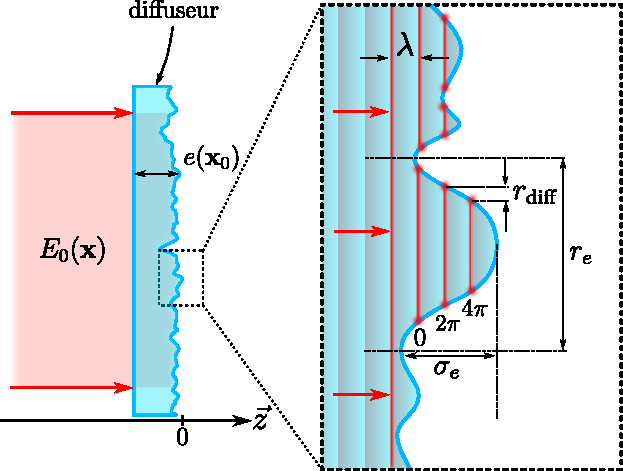
\includegraphics[scale=1]{Fig/Speckle/diffus_prop.pdf}
\label{fig:diffus_prop}
\caption{\textbf{Caractéristiques du diffuseur.} L'épaisseur aléatoire est caractérisée par une hauteur typique $\sigmae$ et une granularité de taille $r_e$. Pour $\sigmae \gg \lambda$, on a plusieurs oscillations de l'onde incidente dans le même grain, et donc $\tdiff$ qui est une fonction $2\pi-$périodique, voit sa corrélation réduite.}
\end{figure}

Les grains du diffuseur sont de plus caractérisés par une certaine extension typique $r_e$ correspondant à une largeur de corrélation de l'épaisseur. Celle-ci induit donc une corrélation spatiale de la transmission, décrite à l'aide la fonction de corrélation
\begin{equation}
\Cdiff(\mathbf{x}_0,\mathbf{x}'_0)=\overline{\tdiff(\mathbf{x}_0)\tdiff^*(\mathbf{x}'_0)}=\overline{e^{i(\phi(\mathbf{x}_0)-\phi(\mathbf{x}'_0))}} { .}
\label{eq:correlation_diffuseur}
\end{equation}

Puisque l'épaisseur et la phase sont proportionnelles, ces deux grandeurs sont corrélées sur la même taille $r_e$ correspondant à la granularité de la surface du verre. En revanche, dans le cas où $\sigmae \gg \lambda$ (ce qui est le cas sur notre expérience), l'onde oscille plusieurs fois dans le même grain du diffuseur. La transmission étant une fonction $2\pi-$périodique de la phase, celle-ci perd alors sa corrélation sur une taille $\rdiff \ll r_e$, voir figure \ref{fig:diffus_prop}. On montre alors annexe \ref{ch:anex_speckle} que la corrélation de la transmission à courte portée\footnote{La corrélation de la transmission tend suffisamment vite vers 0 pour que l'on puisse considérer que $\left|\mathbf{x}_0-\mathbf{x}'_0 \right| \ll r_e$ dans le cas où $\sigma_\phi \gg 2\pi$.} est de forme gaussienne:
\begin{equation}
\Cdiff(\mathbf{x}_0,\mathbf{x}'_0)\approx \exp{\left( -\frac{\left| \mathbf{x}_0 - \mathbf{x}'_0 \right| ^2}{2 \rdiff^2}\right) } \quad \text{avec} \quad \rdiff=r_e/\sigma_\phi \text{ .}
\end{equation}
$\rdiff$ joue alors le rôle de la taille effective d'un émetteur indépendant tel que considéré dans la section \ref{sc:distribution_speckle}. La condition d'un grand nombre d'émetteurs s'écrit alors $\rdiff \ll D$.

Enfin, il est possible de définir l'angle de diffusion $\theta_{\mathrm{diff}}=\lambda/\pi \rdiff=2(n-1) \sigmae/r_e$, qui est indépendant de la longueur d'onde de l'onde laser incidente. $\theta_{\mathrm{diff}}$ est donc une constante du diffuseur, fixée par les paramètres géométriques de celui-ci.










\subsection{Implémentation expérimentale}
Les expériences menées sur notre dispositif jusqu'en 2014 utilisaient un speckle réalisé à la longueur d'onde de \SI{532}{\nano\metre}. Ce grand désaccord vers le bleu par rapport à la transition $\mathrm{D}_2$ du \isotope[87]{Rb} permet ainsi de s'affranchir de l'émission spontanée, même pour les très longs temps de propagation nécessaires à l'étude de la localisation d'Anderson. Depuis 2015 en revanche, l'équipe utilise un speckle accordable autour de \SI{780}{\nano\metre} offrant ainsi la possibilité de réaliser un désordre attractif ou répulsif. Nous verrons section \ref{sc:potentiel_speckle} que cette accordabilité autour de la transition $\mathrm{D}_2$ offre un grand nombre de possibilités expérimentales.

\paragraph*{Mise en forme du faisceau speckle}
Par vœux de concision, seules les grandes lignes du montage de mise en forme du faisceau speckle à \SI{780}{\nano\metre} seront données ici, de nombreux détails à propos de ce montage pouvant être retrouvés dans les thèses de Jérémie Richard, Vincent Denechaud et Musawwadah Mukhtar \citep{richard2015propagation, denechaud2018vers, mukhtar2019state}.

Le faisceau source du speckle est émis par un laser industriel \emph{Toptica TA-Pro} \SI{2}{\watt} accordable autour de \SI{780}{\nano\metre}. Étant donné la proximité de la transition atomique, ce laser est asservi par battements sur le laser repompeur \emph{L2}, ce qui permet d'en fixer la fréquence avec une précision de \SI{1}{\mega\hertz}. Le mode spatial et la polarisation du faisceau sont filtrés à l'aide d'une fibre optique à maintien de polarisation et de cubes séparateurs de polarisation.

La spécificité de ce montage réside dans sa capacité à stabiliser par asservissement une très faible puissance optique, typiquement de quelques \SI{}{\micro\watt} compte-tenu de la proximité de la transition. Pour cela, 90\% de la puissance optique sont déviés vers une photodiode, dont la mesure permet de rétroagir sur la puissance du faisceau à l'aide d'un modulateur acousto-optique. Cette mesure à haute puissance permet de plus d'être particulièrement sensible aux fluctuations de puissance. Le faisceau est ensuite atténué et agrandi avant focalisation sur les atomes et passage au travers du diffuseur. À ce stade, on dispose d'un faisceau de waist \SI{14.6}{\milli\metre} (rayon à $1/e^2$), de polarisation $\pi$ et dont la puissance est stabilisée et contrôlable entre \SI{30}{\nano\watt} et \SI{15}{\micro\watt}.


\paragraph*{Génération du speckle}

\begin{figure}
\centering
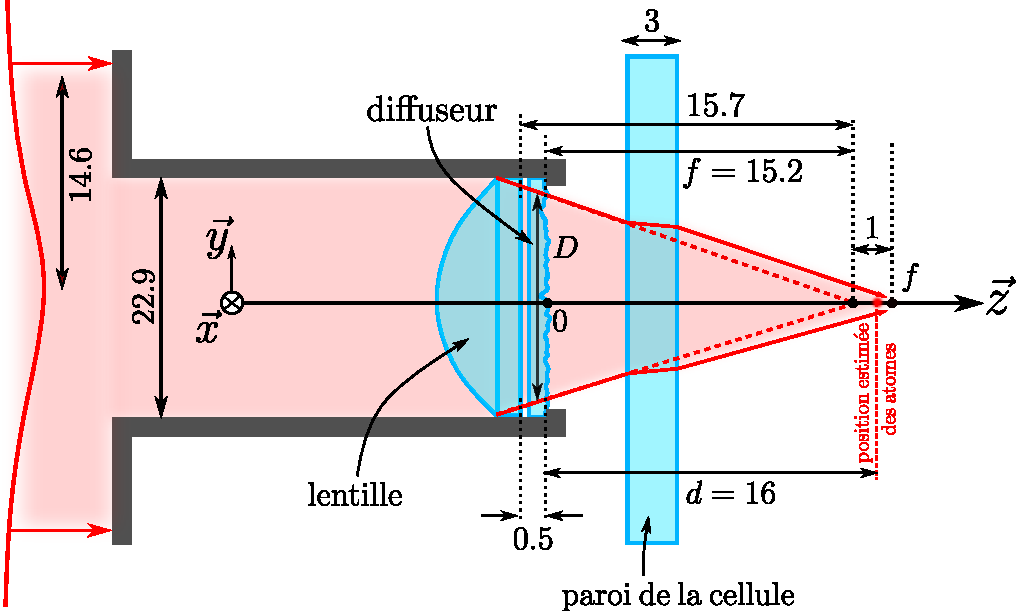
\includegraphics[width=0.9\textwidth]{Fig/Speckle/montage_diffuseur.pdf}
\caption{\textbf{Géométrie du montage de génération du speckle.} Un faisceau gaussien incident de waist \SI{14.6}{\milli\metre} est tronqué dans un diaphragme de diamètre \SI{22.9}{\milli\metre} qui supporte le diffuseur. Ce faisceau est ensuite focalisé par une lentille asphérique épaisse de focale \SI{16}{\milli\metre} et traverse le diffuseur d'épaisseur \SI{0.3}{\milli\metre}. Le plan de focalisation est déplacé d'environ \SI{1}{\milli\metre} à cause de la paroi de la cellule à vide, d'épaisseur \SI{3}{\milli\metre}.}
\label{fig:montage_diffuseur}
\end{figure}

La génération du speckle se fait selon le montage représenté figure \ref{fig:montage_diffuseur}. Un faisceau gaussien collimaté de waist \SI{14.6}{\milli\metre} et de longueur d'onde $\lambda=\SI{780}{\nano\metre}$, dont la mise en forme a été présentée dans le paragraphe précédent, est tronqué par un diaphragme de diamètre \SI{22.9}{\milli\metre}. Ce faisceau passe ensuite au travers d'une lentille asphérique épaisse (\textit{Thorlabs ACL2520-B}) de focale \SI{16.0}{\milli\metre} (et de frontale \SI{15.7}{\milli\metre}) montée dans ce même diaphragme. Le rôle de celle-ci est de focaliser la lumière sur les atomes\footnote{Nous verrons dans la section suivante que cela permet d'obtenir des grains de speckle les plus petits possibles. En effet, on attend la manifestation d'effets quantiques sur la propagation d'une onde de matière dans un speckle pour des longueurs d'onde de de Broglie plus grandes que la taille des grains de speckle.}. Accolé à cette lentille se trouve un diffuseur \textit{Newport FSD10-3} possèdant une épaisseur de \SI{0.3}{\milli\metre}\footnote{Cette épaisseur était initialement de \SI{3}{\milli\metre} avant d'être réduite à \SI{0.3}{\milli\metre} par l'atelier d'optique de l'IOGS.} et un angle de diffusion $\theta_{\mathrm{diff}}\approx\SI{5}{\degree}$. 

Enfin, ce faisceau convergent traverse la paroi de la cellule en verre sous ultra-vide d'épaisseur $e=\SI{3.0}{\milli\metre}$ et située à \SI{0.5}{\milli\metre} de la monture du diffuseur. Le matériau de cette cellule est du Vycor, d'indice optique $n=1.46$. L'épaisseur de cette cellule, considérée comme une lame à faces parallèles, induit un décalage des rayons lumineux par réfraction, décalage représenté figure \ref{fig:montage_diffuseur} montrant la trajectoire des rayons lumineux en absence de la paroi par des traits pointillés. La présence de la paroi entraîne donc un déplacement du plan de focalisation donné par $\Delta d=e(1-1/n)\approx \SI{1}{\milli\metre}$. La distance focale en présence de la paroi de la cellule est alors de \SI{17.0}{\milli\metre}.


En choisissant pour origine de l'axe $\vec{z}$\footnote{L'axe $\vec{z}$ utilisé dans ce chapitre correspond à la direction de propagation du faisceau speckle. Dans le repère de l'expérience, il s'agit en réalité de l'axe $\vec{x}$, perpendiculaire au plan formé par les faisceaux du piège optique.} la surface du diffuseur, la position du plan de focalisation se trouve à $f=\SI{16.4}{\milli\metre}$. Dans ce repère, la position des atomes dans le piège optique est estimée quant à elle a $d=16\pm\SI{0.5}{\milli\metre}$, dont la valeur est proche de celle de la position du plan de focalisation. Néanmoins, l'incertitude liée à la position des atomes est cruciale, celle-ci pouvant conduire à un écart de \SI{0.9}{\milli\metre} du plan de focalisation. Il est ainsi primordial de connaître les propriétés du speckle autour du plan de focalisation. 









\section{Propriétés spatiales d'un champ de speckle}
\label{sc:speckle_correlation}

Le speckle résultant de la propagation d'un faisceau transmit par le diffuseur, il est donc régit par les lois de la diffraction et il est possible de déduire ses propriétés spatiales de celles de l'éclairement au niveau au diffuseur. Notamment, les variations spatiales du champ de speckle sont décrites quantitativement par la fonction de corrélation de ce champ. L'étude de cette fonction de corrélation nous permet donc de déterminer toutes les tailles caractéristiques d'intérêt pour notre expérience, l'extension du champ de speckle ainsi que les tailles moyennes des grains de lumière. 

Dans cette section, nous allons nous attacher à décrire ces échelles de longueur caractéristiques autour du plan de focalisation à l'aide de la fonction de corrélation du champ, dont le détail des calculs est donné en annexe \ref{ch:anex_speckle}. 

De plus, lors de la conception de ce système, l'extension du champ de speckle ainsi que les tailles des grains de speckle ont été mesurées expérimentalement sur un montage reproduisant exactement les conditions réelles en présence de la cellule à vide, celle-ci empêchant de faire des mesures in-situ. La description de ces mesures et de leur traitement sont référencées dans la thèse de Jérémie Richard \citep{richard2015propagation}.




\subsection{Extension transverse du champ de speckle le long le l'axe optique}
L'extension transverse du champ de speckle est donnée par le waist du faisceau speckle, il est donc nécessaire de calculer le profil d'intensité moyenne $\overline{I}(\xd)$, où l'ensemble des points $\lbrace\xd\rbrace$ correspond au plan $\lbrace x,y,z=d \rbrace$ situé à une distance $d$ de la surface du diffuseur. Pour cela, explicitons le champ rayonné $E(\xd)$ à l'aide du principe de Huygens-Fresnel dans l'approximation paraxiale:
\begin{equation}
E(\xd) \propto \int{\mathrm{d}\xzero \: \Ediff (\xzero) \exp{\left( ik\frac{\xzero^2}{2\deff} \right) } \: \exp{\left( -ik \frac{\xd \cdot \xzero}{d} \right) } } \text{ ,}
\label{eq:amplitude_rayonnee}
\end{equation}
où $k=2\pi/\lambda$ est le nombre d'onde et $\deff$ correspond à une distance effective donnée par $1/\deff=1/d-1/f$. L'ensemble des points $\lbrace\xzero\rbrace$ décrit le plan du diffuseur $\lbrace x,y,z=0 \rbrace$, et $\Ediff (\xzero)$ correspond au champ dans ce plan, qu'il est possible de décomposer sous la forme 
\begin{equation}
\Ediff(\xzero)=\Ezero(\xzero) \tdiff(\xzero) \quad \text{avec} \quad \Ezero(\xzero) = E_\mathrm{inc} (\xzero) m(\xzero) \text{ ,}
\end{equation}
où $\tdiff(\xzero)$ est la transmission du diffuseur, $E_{\mathrm{inc}}(\xzero)$ est le champ incident\footnote{Il s'agit du faisceau gaussien de waist \SI{14.6}{\milli\metre}.}, et $m(\xzero)$ est un masque représentant le diaphragme et les montures de optiques. On écrira $m(\xzero)$ comme étant une pupille de diamètre $D$. $\Ezero(\xzero)$ correspond alors au champ au niveau du diffuseur, et on supposera dans la suite que celui-ci varie lentement à l'échelle des variations de $\tdiff(\xzero)$, c'est à dire que $\Ezero(\xzero+\delta\xzero)\approx\Ezero(\xzero)$ avec $\delta\xzero$ de l'ordre de $\rdiff$.

On montre alors (voir annexe \ref{ch:anex_speckle}) que le profil d'intensité moyenne à la distance $d$ peut s'écrire
\begin{align}
\nonumber\overline{I}(\xd)&=\overline{E(\xd) E^*(\xd)} \\
&\propto I_0 \left( \frac{\deff}{d} \xd \right) \ast \widetilde{\Cdiff}\left( \frac{\xd}{\lambda d} \right) \text{ ,}
\end{align}
où le symbole $\ast$ dénote le produit de convolution. L'évolution du profil d'intensité moyenne en fonction de la distance $d$ est alors dû à deux contributions dont l'interprétation physique est la suivante:
\begin{itemize}
\item[\textendash] Le premier terme correspond à l'effet de la lentille, et focalise donc le profil d'intensité initiale $I_0(\xzero)=\left| \Ezero(\xzero) \right|^2$ dans le plan focal $\lbrace x,y,z=f\rbrace$. Cette focalisation se traduit au travers d'un changement d'échelle de l'intensité par le facteur $d/\deff=\left| d-f \right| /f$. Ainsi, la taille de ce faisceau focalisé décroît avec la distance jusqu'à s'annuler dans le plan focal, comme prédit par l'optique géométrique.
\item[\textendash] Le second terme est la transformée de Fourier de la fonction de corrélation du diffuseur $\Cdiff(\xzero)$. Ce terme traduit la diffraction de l'onde incidente par les grains du diffuseur de taille $\rdiff$, dont la largeur est donnée par $\lambda d/ \pi \rdiff$, qui croît linéairement avec la distance $d$.
\end{itemize}
Ces dépendances sont illustrées figure \ref{fig:speckle_extension}, où le fond rose correspond au premier terme de focalisation, tandis le fond orange illustre le second terme de diffraction. On identifie alors deux régimes pour lesquels un terme est prépondérant. 

\begin{figure}
\centering
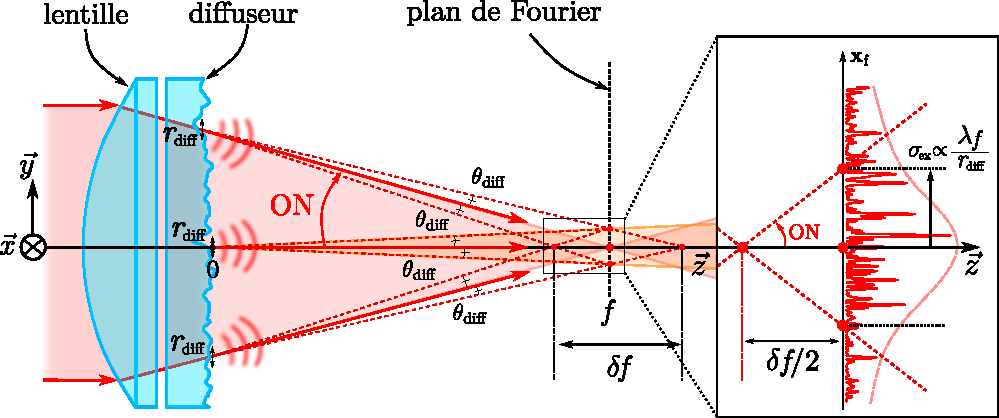
\includegraphics[width=\textwidth]{Fig/Speckle/speckle_extension.pdf}
\caption{\textbf{Extension du champ de speckle.} L'extension du faisceau de speckle est due à deux effets distincts, la focalisation du faisceau incident et la diffraction du faisceau par le diffuseur. La contribution de la focalisation à l'extension du faisceau est illustrée par des flèches rouges et un remplissage rose, tandis que celle de la diffraction correspond à un remplissage orange. La région aux alentours du plan focal est particulièrement intéressante car il s'agit de celle où l'ensemble des émetteurs contribuent à l'éclairement, chaque émetteur diffractant dans un cône d'angle $\theta_{\mathrm{diff}}$ illustré par des pointillés rouges. Dans le cas où l'angle de diffusion est petit devant l'ouverture numérique $\theta_{\mathrm{diff}} \ll \ON$, on peut estimer par trigonométrie l'étendue de cette région à $\delta f/2= \speckleext / \ON$ (encart).}
\label{fig:speckle_extension}
\end{figure}

Dans une première région, loin du plan focal de la lentille, la taille du faisceau est donnée par l'effet de focalisation de la lentille. Une seconde région, proche du plan focal de la lentille, est dominée par l'effet de diffraction des émetteurs du diffuseur, la taille de l'éclairement incident étant fortement réduite par focalisation. Ainsi, pour une zone très proche du plan focal de la lentille, on peut décrire le profil d'intensité lumineuse par 
\begin{equation}
\overline{I}\propto \mathrm{TF} \left[ \Cdiff \right] (\xf/\lambda f)
\end{equation}
où l'ensemble des points $\lbrace \xf \rbrace$ correspond au plan de Fourier\footnote{Dans le plan focal $\lbrace x,y,z=f\rbrace$, le champ rayonné est alors la transformée de Fourier du champ incident comme illustré par la formule \ref{eq:amplitude_rayonnee}. Il s'agit d'une propriété bien connue des lentilles de pouvoir ramener l'infini de la diffraction de Fraunhofer à distance finie.} $\lbrace x,y,z=f \rbrace$, et $\Cdiff$ est la fonction de corrélation du diffuseur, de forme de gaussienne avec une largeur $\rdiff$. Le profil d'intensité lumineuse dans le plan de Fourier est alors donnée par 
\begin{equation}
\overline{I}(\xf)\propto \exp{(-\frac{2 \left| \xf \right|^2}{\speckleext})} \quad \text{avec} \quad \speckleext = \frac{\lambda f}{\pi \rdiff} \text{ .}
\label{eq:intensite_moyenne_speckle}
\end{equation}
$\speckleext$ correspond donc au waist du profil d'intensité moyenne, dont l'expression peut se réécrire à l'aide de l'angle du diffusion $\speckleext=\theta_{\mathrm{diff}} f = 1.5\pm\SI{0.1}{\milli\metre}$. Donc, dans le plan de Fourier, l'extension du champ de speckle ne provient que de l'effet de la diffraction des émetteurs individuels dont les faisceaux se recouvrent tous, comme illustré figure \ref{fig:speckle_extension} par la zone orange.

Cette condition de recouvrement des faisceaux provenant de l'ensemble des émetteurs du diffuseur permet de considérer que dans cette région le speckle est entièrement développé. Afin d'en déterminer l'étendue longitudinale, on s'intéresse aux positions de l'espace où l'ensemble des faisceaux provenant du diffuseur participent. Dans la limite $\theta_{\mathrm{diff}} \ll \ON$, on détermine par trigonométrie que cette zone s'étend par part et d'autre du plan de Fourier sur une distance $\delta f/2\approx \speckleext /\ON =2.5\pm\SI{0.1}{\milli\metre}$ (voir figure \ref{fig:speckle_extension}), délimitant ainsi les régions décrites précédemment. Par analogie avec un faisceau gaussien, on appellera $\delta f$ \emph{distance de Rayleigh} du champ de speckle, et sa valeur nous assure que les atomes de trouveront dans la zone où le speckle est pleinement développé, celle-ci étant un ordre de grandeur plus grande que l'incertitude de positionnement des atomes.















\subsection{Longueur de corrélation transverse le long de l'axe optique}
La seconde taille caractéristique du speckle, la taille des grains de lumière, est une grandeur d'une importance capitale pour la physique du désordre. Si l'extension du faisceau de speckle est une grandeur d'intérêt pratique (celle-ci donne une borne supérieure sur les tailles de nuages), nous verrons chapitre \ref{ch:TauS_PRL} que la taille des grains de speckle fixe la dynamique de la propagation d'une onde en milieu désordonné.

La taille de ces grains est donnée par la largeur de la fonction de corrélation des fluctuations d'intensité, le potentiel ressenti par les atomes étant proportionnel à l'intensité lumineuse. À l'aide du théorème de Wick pour les variables gaussiennes, il est possible de relier cette fonction de corrélation des fluctuations d'intensité à la fonction de corrélation en amplitude du champ:
\begin{equation}
\overline{\delta I(\xd) \delta I(\xd')} = \left| \overline{E(\xd)E^*(\xd')} \right|^2 \text{ ,}
\end{equation}
où $\delta I(\xd)=I(\xd)-\overline{I}(\xd)$ correspond aux fluctuations statistiques d'intensité et les positions $\xd$ et $\xd'$ correspondent à deux points dans le plan $\lbrace x,y,z=d\rbrace$ transverse à l'axe optique. 


Dans les conditions expérimentales usuelles, il est possible de négliger l'effet de l'extension spatiale finie du speckle, celle-ci étant très grande à l'échelle des grains de speckle. Ainsi, on peut considérer que la fonction de corrélation en amplitude ne dépend uniquement que de la différence des positions considérées. Dans ce régime, on montre annexe \ref{ch:anex_speckle} que la fonction de corrélation transverse en amplitude le long de l'axe optique peut s'écrire:
\begin{align}
\nonumber \CE(\xd,\xd') &= \overline{E(\xd) E^*(\xd')} \\
& \propto \widetilde{I_0}\left( \frac{\delta\xd}{\lambda d}\right) \ast \Cdiff\left( \frac{\deff}{d} \delta \xd \right) \text{ ,}
\label{eq:correlation_transverse_speckle}
\end{align}
où $\delta\xd=\xd'-\xd$. De même que pour l'extension spatiale du champ de speckle, la fonction de corrélation transverse résulte de deux contributions, dont les interprétations physiques sont les suivantes:
\begin{itemize}
\item[\textendash] Le premier terme correspond à la transformée de Fourier de l'intensité lumineuse dans le plan du diffuseur. Il s'agit ici du motif de diffraction à l'infini en l'absence du diffuseur, dont la taille est proportionnelle à la distance. Ce facteur d'échelle s'interprète comme une diminution de l'ouverture numérique au fur et à mesure de l'éloignement avec le diffuseur, comme indiqué par la relation $\ON'(d)=D/2d$, avec $D$ la taille typique de l'éclairement au niveau du diffuseur. Ce terme conduit donc à largeur de l'ordre de $\sim\lambda / \pi \ON'(d)$, qui croît linéairement avec la distance $d$. 
\item[\textendash] Le second terme décrit quant à lui le fait que les grains du diffuseur ne diffractent que selon un angle $\theta_{\mathrm{diff}}$. De fait, ce terme décrit les régions de l'espace dans lesquelles l'ensemble du diffuseur ne participe pas à l'interférence au point $\xd$. Ce terme joue ainsi le rôle d'ouverture numérique effective, dont l'expression $\ON_{\mathrm{eff}}(d)=\theta_{\mathrm{diff}} f/\left| d-f \right|$ peut être obtenue par trigonométrie. L'écriture de ce terme donnée équation \ref{eq:correlation_transverse_speckle} permet néanmoins d'obtenir une expression simple de la largeur induite pour la fonction de corrélation transverse: $\sim\lambda /\pi \ON_{\mathrm{eff}} (d)$.
\end{itemize}
La largeur de la fonction de corrélation apparaît alors comme la plus petite taille permise par les lois de la diffraction: il s'agit de la limite de diffraction. L'étude des grains de speckle se résume alors à l'évolution de l'ouverture numérique le long de l'axe de propagation du faisceau.

À l'instar de l'extension du champ de speckle, il est possible d'identifier deux régions dans lesquelles le comportement de la largeur de la fonction de corrélation transverse en amplitude du speckle est majoritairement dû à l'un des effets mentionnés ci-dessus. La frontière entre ces deux régions est donnée, comme pour l'extension du speckle, par la distance de Rayleigh qui caractérise, rappelons-le, l'étendue sur laquelle l'ensemble de diffuseur participe à l'amplitude rayonnée.

Les atomes se trouvant à proximité du plan de Fourier, la fonction de corrélation sera donc dominée par le régime de diffraction à l'infini, où l'ouverture numérique y est maximale. La fonction de corrélation des fluctuations d'intensité s'écrit alors simplement
\begin{equation}
\overline{\delta I (\xf) \delta I (\xf + \delta \xf)} \propto \left| \mathrm{TF} \left[ I_0 \right] (\delta \xf / \lambda f \right| ^2 \text{ .}
\end{equation}
La forme de la fonction de corrélation aux alentours du plan de Fourier nécessite tout de même une connaissance fine du profil d'intensité dans le plan du diffuseur. 

Nous retiendrons ici que la taille transverse des grains de lumière est donnée par la limite de diffraction du système, $\sigmap\sim \lambda/\pi\ON$ de l'ordre de \SI{0.5}{\micro\metre}, bien inférieure à l'extension du faisceau de speckle $\sigmap \ll \speckleext$. Une calibration précise de la taille transverse des grains de speckle est présentée section \ref{sc:speckle_non_paraxial}.




\subsection{Longueur de corrélation longitudinale autour du plan de Fourier}

On peut montrer que la corrélation longitudinale en amplitude aux alentours du plan de Fourier s'écrit
\begin{equation}
\overline{E(f)E^*(f+\delta z)} \propto \int{\mathrm{d} \xzero I_0 (\xzero) e^{i\pi \xzero^2 \delta z / \lambda f^2} } \text{ .}
\end{equation}
De même que pour la fonction de corrélation transverse proche du plan de Fourier, celle-ci ne dépend que de l'éclairement incident dont la forme est celle d'une gaussienne tronquée par un diaphragme dont le rayon légèrement plus grand que le waist du faisceau.

Dans le cas d'un éclairement purement gaussien, la corrélation longitudinale des fluctuations d'intensité est de forme lorentzienne:
\begin{equation}
\overline{\delta I(f) \delta I(f+\delta z)} = \overline{\delta I^2} \frac{1}{1+\delta z^2 / \sigmal^2}
\end{equation}
avec $\sigmal=\sigmap/\ON$



Calculs de la corrélation longitudinale. Formule de la thèse de Fred redémontrée en annexe. Application à un éclairement gaussien, et un éclairement homogène tronqué. Réalité entre les deux, donc la fonction de corrélaiton réelle est quelque part entre une lorentzienne et un sinus cardinal. 





\subsection{Effets non-paraxiaux sur les corrélations du speckle}
\label{sc:speckle_non_paraxial}
C'est pas parfait partout, alors modélisation en tenant compte des effets non-paraxiaux pour vraiment reproduire la corrélation longitudinale. Calculs lourds numériquement et théoriquement, donc on met en place un modèle paraxial à ON effective. Avecun facteur de scaling sur la taille du faisceau incident et sur la pupille, on arrive à reproduire de manière convenable la corrélation longitudinale. Avantage: ça reste paraxial donc on peut en tirer des grandeurs. 






\section{Propriétés du potentiel de type speckle}
\label{sc:potentiel_speckle}
Jusqu'à ce point, nous nous sommes attachés à décrire le champ lumineux d'un speckle. En particulier, nous avons montré le montré le caractère granulaire de celui-ci, granularité dont la taille est donnée par la limite de diffraction. 

À présent, nous allons décrire comment les propriétés du champ de speckle se traduisent en terme de potentiel pour les atomes. 

\subsection{Propriétés du potentiel}
\label{sc:propriete_potentiel_speckle}
Comme annoncé en introduction de ce chapitre, le désordre nécessaire à l'étude de la propagation d'ondes de matière en milieux désordonnés est réalisé à l'aide du champ de speckle décrit précédemment, dont l'effet sur les atomes est décrit par le potentiel dipolaire présenté section \ref{sc:forces_lumineuses}. En effet, l'effet d'un champ laser de pulsation $\omega$ et d'intensité $I(\mathbf{x})$ sur un atome à deux niveaux séparés par $\hb \omega_0$ est donné par \ref{eq:potentiel_dipolaire}, que l'on peut écrire plus simplement 
\begin{equation}
V(\mathbf{x}) \propto I(\mathbf{x}) \left( \frac{1}{\omega-\omega_0} - \frac{1}{\omega+\omega_0} \right) \text{ .}
\end{equation}
Comme décrit précédemment, le laser utilisé pour créer ce champ de speckle est accordable autour de \SI{780}{\nano\metre}, c'est à dire proche de la résonance de la raie $D_2$ du \isotope[87]{Rb}. Dans ces conditions, il est possible d'appliquer l'approximation de l'onde tournante et de négliger le terme en $1/(\omega+\omega_0)$ devant le terme co-rotatif en $/(\omega-\omega_0)$, le potentiel ressenti par les atomes s'exprimant alors
\begin{equation}
V(\mathbf{x}) \propto \frac{I(\mathbf{x})}{\delta} \text{ ,}
\label{eq:potentiel_dipolaire_approx}
\end{equation}
où $\delta=\omega-\omega_0$ est le désaccord du faisceau par rapport à la transition. 

Le potentiel désordonné ressenti par les atomes étant proportionnel à l'intensité lumineuse, il apparaît alors que les propriétés statistiques spatiales du potentiel sont exactement celles de l'intensité lumineuse du speckle. Notamment, le potentiel généré par un speckle est anisotrope et la taille typique des fluctuations de potentiel aux alentours du plan de Fourier est donnée par $\sigmap=\SI{0.5}{\micro\metre}$ dans le plan transverse et $\sigmal=\SI{4.1}{\micro\metre}$ dans la direction longitudinale, les fonctions de corrélations du potentiel et de l'intensité lumineuse étant identiques.

De plus, il a été montré dans la section précédente que le champ de speckle n'est pas homogène, mais qu'il possède une extension finie. En particulier, l'équation \ref{eq:intensite_moyenne_speckle} stipule que le profil d'intensité moyenne est une gaussienne de waist $\speckleext\approx \SI{1.5}{\milli\metre}$, dont l'intensité au centre du faisceau dépend la puissance du laser $P$ selon
\begin{equation}
\overline{I}(\xf=0)=\frac{2P}{\pi \speckleext^2} \text{ ,}
\end{equation}
d'après les lois de l'optique gaussienne. Les tailles typiques des nuages utilisés étant au maximum de quelques dizaines de \SI{}{\micro\metre}, on peut supposer qu'à cette échelle, le potentiel moyen ressenti par les atomes est homogène et que sa valeur est fixée par l'intensité lumineuse au centre de la figure de speckle: $\VR=\overline{V} \propto \overline{I}(\xf=0)/\delta$.

Une autre conséquence de l'expression \ref{eq:potentiel_dipolaire_approx} est qu'il est possible de créer un potentiel désordonné sur les atomes qui soit répulsif ($\delta>0$) ou bien attractif ($\delta<0$) selon le signe du désaccord $\delta$. Cette dernière possibilité nous permet d'avoir un degré de liberté expérimental supplémentaire, celui de la distribution de potentiel, dont l'importance sera illustrée dans les chapitres \ref{ch:TauS_PRL} et \ref{ch:TauS_NJP}. En effet, si la distribution de la norme du potentiel est fixée par celle de l'intensité lumineuse \ref{eq:proba_speckle}, ces deux quantités étant proportionnelles, le signe du désaccord nous permet de retourner la distribution de potentiel par rapport au potentiel nul $V=0$ (voir figure \ref{fig:distribution_potentiel})
\begin{equation}
\mathcal{P}(V)=\frac{1}{\left| \VR \right|} e^{-V/\VR} \cdot \Theta(V/\VR) \text{ ,}
\end{equation}
où $\Theta$ est la fonction de Heaviside valant 1 pour $V/\VR>0$, et 0 sinon. $\VR$ est le potentiel moyen, proportionnel à l'intensité lumineuse moyenne et dont le signe peut changer suivant celui du désaccord. L'amplitude du désordre est quant à elle donnée par l'écart-type de la distribution de potentiel $ \sigma_{V}=(\overline{V^2}-\overline{V}^2)^{1/2}=\left|\VR\right|>0$ et sera toujours positive. Ainsi, sur notre dispositif, changer l'amplitude du désordre revient simplement à faire varier la puissance du faisceau speckle rayonné sur les atomes.


\begin{figure}
\centering
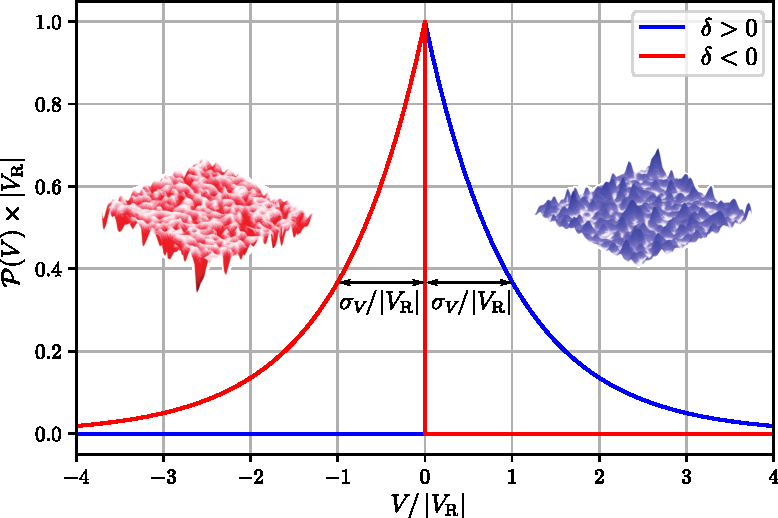
\includegraphics[width=0.95\textwidth]{Fig/Speckle/distribution_potentiel.pdf}
\caption{\textbf{Distributions de potentiel pour un désordre optique de type speckle.} La distribution de potentiel suit celle de l'intensité lumineuse. Pour des désaccords positifs $\delta>0$, le potentiel créé est positif et sa distribution est une exponentielle décroissante (courbe bleue). Pour des désaccords négatifs $\delta<0$, le potentiel est alors attractif et ne peut dépasser 0. La distribution de potentiel est alors une exponentielle croissante (courbe en rouge).}
\label{fig:distribution_potentiel}
\end{figure}






\subsection{Possibilité d'un potentiel dépendant de l'état interne}
L'étude de la transition d'Anderson, en particulier du régime critique, nécessite de pouvoir adresser sélectivement les différents niveaux d'énergie liés au désordre. Il s'agit donc de procéder à une spectroscopie du désordre. Pour cela, nous devons disposer d'un état libre dans lequel nous préparons notre condensat de Bose-Einstein, c'est à dire insensible au potentiel désordonné, et d'un second état couplé au désordre.Dans cette section, on s'attachera donc à décrire la notion de potentiel dépendant de l'état interne des atomes.

\paragraph*{Principe du désordre dépendant de l'état interne}
Comme explicité section \ref{sc:forces_lumineuses}, la formule \ref{eq:potentiel_dipolaire} décrivant le potentiel dipolaire a été obtenue dans la limite des grands désaccords pour un système à deux niveaux, ne tenant donc pas compte ni de la structure fine, ni de la structure hyperfine du \isotope[87]{Rb}. En particulier, la structure hyperfine de l'état fondamental $5^2S_{1/2}$ possède deux niveaux $\etatF{1}{}$ et $\etatF{2}{}$ séparés de $\deltahf=\SI{6.83}{\giga\hertz}$ très grande devant la largeur de la transition $\Gamma/2\pi=\SI{6.07}{\mega\hertz}$. 

En fixant le désaccord $\delta_{\mathrm{2,F'}}$ par rapport à la transition $\etatF{2}{}\rightarrow \etat{F'}$ de telle sorte que celui-ci soit très petit devant la séparation hyperfine des états fondamentaux $\left| \delta_{\mathrm{2,F'}} \right| /2 \pi \ll \deltahf$, on peut réaliser un potentiel dont la valeur moyenne dépend de l'état interne:
\begin{equation}
\overline{V_2} \propto \frac{\overline{I}}{\delta_{\mathrm{2,F'}}} \quad \text{et} \quad \overline{V_1} \propto \frac{\overline{I}}{\delta_{\mathrm{2,F'}}+\deltahf} \text{ .}
\end{equation}
Avec la condition d'un petit désaccord, on obtient alors $\left| \overline{V_1} \right| \ll \left| \overline{V_2} \right|$, comme illustré figure \ref{fig:principe_potentiel_etat_interne}. On dispose donc d'un moyen de réaliser un potentiel conséquent sur l'état $\etatF{2}{}$ tout en perturbant peu l'état $\etatF{1}{}$ dans lequel on prépare notre condensat de Bose-Einstein.


\begin{figure}
\centering
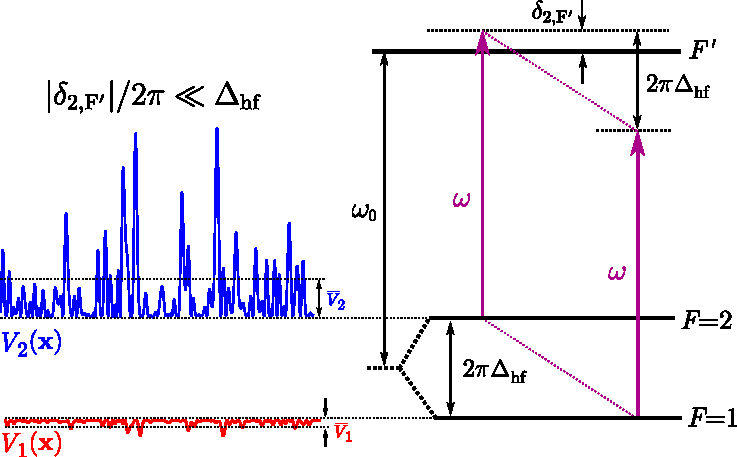
\includegraphics[width=0.85\textwidth]{Fig/Speckle/principe_potentiel_etat_interne.pdf}
\caption{\textbf{Réalisation d'un potentiel dépendant de l'état interne.} Le choix d'un désaccord par rapport à la transition $\protect\etatF{2}{} \rightarrow \protect\etat{F'}$ qui soit petit devant la séparation hyperfine des états $\protect\etatF{1}{}$  et $\protect\etatF{2}{}$ permet de soumettre un potentiel aux atomes dans l'état $\protect\etatF{2}{}$ tout en perturbant peu ceux dans l'état $\protect\etatF{1}{}$. Plus de blabla ici.}
\label{fig:principe_potentiel_etat_interne}
\end{figure}


\paragraph*{Détails du potentiel dipolaire}
Cependant, à l'échelle des désaccords typiques recherchés dans une telle situation (de l'ordre de \SI{100}{\mega\hertz}), il est aussi nécessaire de tenir compte de la structure hyperfine de l'état excité $5^2 P_{3/2}$ du \isotope[87]{Rb}, qui se décompose en quatre états hyperfins $\etat{F'=\lbrace 0,1,2,3 \rbrace}$. On peut alors montrer que le potentiel dipolaire ressenti par les états fondamentaux $\etatF{1}{}$ et $\etatF{2}{}$ est la somme des contributions de chacune des transitions vers un état excité \citep{grimm1999optical}. 

De plus, le faisceau speckle étant polarisé linéairement suivant l'axe du champ magnétique $\vec{y}$, les contributions au potentiel dipolaire se restreignent aux transitions $\pi$ ($\Delta\mf=0$) et on peut alors montrer à l'aide d'un calcul attentif de la polarisabilité atomique que le potentiel dipolaire ressenti par les états fondamentaux hyperfins est donné par \citep{grimm1999optical}\citep{steck2001rubidium}\citep{denechaud2018vers}:
\begin{equation}
V_2(\mathbf{x}) = \frac{3 \pi c^2 \Gamma I(\mathbf{x})}{\omega_0^3} \left( \frac{1}{40 \: \delta_{2,1}} + \frac{1}{24 \: \delta_{2,2}} + \frac{4}{15 \: \delta_{2,3}} \right) 
\label{eq:potentiel_dipolaire_hyperfin_V2}
\end{equation}
et
\begin{equation}
V_1(\mathbf{x}) = \frac{3 \pi c^2 \Gamma I(\mathbf{x})}{\omega_0^3} \left( \frac{5}{24 \: \delta_{1,1}} + \frac{1}{8 \: \delta_{1,2}} \right) \text{ ,}
\label{eq:potentiel_dipolaire_hyperfin_V1}
\end{equation}
où les $\delta_{\mathrm{F,F'}}$ correspondent aux désaccords en \SI{}{\radian\per\second} associés à chacune des transitions $\etat{F,\mf} \rightarrow \etat{F',\mf'=\mf}$. En prenant la transition $\etat{F=2} \rightarrow \etat{F'=3}$ comme référence, on peut tracer l'évolution du potentiel dipolaire pour l'état $\etat{F=2}$ en fonction du désaccord $\delta_{2,3}$, les autres désaccords étant déductibles de la structure hyperfine des états excités. Cette évolution est représentée figure \ref{fig:potentiel_dipolaire_hyperfin}, qui comporte trois divergences du potentiel correspondant aux trois transitions $\pi$ possibles $\etat{F=2} \rightarrow \etat{F'=\lbrace 1,2,3 \rbrace}$.


\begin{figure}
\centering
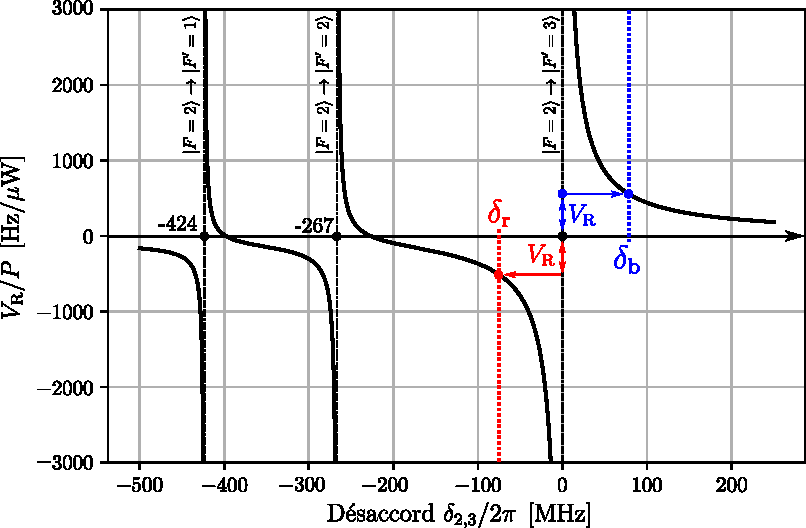
\includegraphics[width=0.9\textwidth]{Fig/Speckle/potentiel_dipolaire_hyperfin.pdf}
\caption{\textbf{Potentiel dipolaire dû à la structure hyperfine du \isotope[87]{Rb}.} En fixant la puissance du faisceau speckle d'extension $\speckleext$, le potentiel moyen $\VR$ ressenti par l'état $\protect\etatF{2}{}$ évolue avec le désaccord $\delta_{2,3}$ par rapport à la transition $\protect\etatF{2}{} \rightarrow \etat{F'=3}$. Les trois divergences de potentiel observées correspondent aux trois transitions $\pi$ possibles.}
\label{fig:potentiel_dipolaire_hyperfin}
\end{figure}

À l'instar du cas d'un potentiel réalisé à l'aide d'un désaccord suffisamment grand devant la structure hyperfine du \isotope[87]{Rb} présenté dans la section \ref{sc:propriete_potentiel_speckle} précédente, la figure \ref{fig:potentiel_dipolaire_hyperfin} illustre la possibilité de réaliser des potentiels qui soient attractifs ou répulsifs en sélectionnant soigneusement le désaccord du laser par rapport à la transition $\etat{F=2} \rightarrow \etat{F'=3}$\footnote{La sélection de cette transition comme référence s'explique par sa forte contribution au potentiel ressenti par l'état $\protect\etatF{2}{}$ comme explicité équation \ref{eq:potentiel_dipolaire_hyperfin_V2}. Ceci est aussi visible sur la figure \ref{fig:potentiel_dipolaire_hyperfin} où l'effet de cette transition apparaît sur une bande d'environ $\pm\SI{200}{\mega\hertz}$, bien plus large que pour les deux autres transitions.}. Dans cet exemple, les désaccords $\delta_{2,3}=\delta_{\mathrm{r}}=-2\pi \times \SI{73}{\mega\hertz}$  et $\delta_{2,3}=\delta_{\mathrm{b}}=2\pi \times \SI{81}{\mega\hertz}$ choisis permettent tous deux d'obtenir un potentiel moyen $\left|\VR\right| /P=h\times\SI{0.53}{\kilo\hertz/\micro\watt}$ où $\VR=\overline{V_2}$ est le potentiel moyen ressenti par l'état $\etat{F=2}$. Le choix de tels désaccords pour des désordres attractifs ($\delta_{\mathrm{r}}<0$) ou bien répulsifs ($\delta_{\mathrm{b}}>0$) donne alors un rapport de potentiels sur les états $\etatF{1}{}$ et $\etatF{2}{}$ de l'ordre de 
\begin{equation}
\left|V_1 \right| / \left| V_2 \right| \approx 0.01 \text{ ,}
\label{eq:ratio_desordre_etat}
\end{equation}
montrant donc la très forte différence entre les potentiels ressentis par les deux états fondamentaux de notre atome. La mise en œuvre expérimentale d'un tel désordre dépendant de l'état interne des atomes a permit la mesure des fonctions spectrales \citep{volchkov2018measurement}, dont les grandes lignes de ce procédé seront décrites dans le chapitre \ref{ch:TauS_NJP}. L'ensemble des détails de ces mesures est documenté dans la thèse de Vincent Denechaud \citep{denechaud2018vers}.




\paragraph*{Limitation du potentiel résiduel sur l'état $\etatF{1}{}$}
Une conséquence de l'équation \ref{eq:ratio_desordre_etat} est la suivante. Bien que le potentiel moyen $\overline{V_1}$ ressenti par l'état $\etatF{1}{}$ soit faible, celui-ci ne s'annule pas exactement. Quelle limite peut-on alors donner à la force du désordre $\VR$? Pour ça on s'intéresse à la limite que l'on peut donner au potentiel résiduel $V_1$. 


Nous avons vu section \ref{sc:propriete_BEC} que pour un condensat de Bose-Einstein dans le régime de Thomas-Fermi, les interactions entre particules écrantent le potentiel externe soumis aux atomes. Il en résulte que sur l'ensemble du condensat, l'énergie des atomes est constante et égale au potentiel chimique $\mu$. Ainsi, pour un potentiel désordonné résiduel d'amplitude faible $\overline{V_1}\ll\mu$, une petite modulation de densité du condensat permet de compenser l'effet de ce potentiel. Ainsi, l'énergie potentielle de chaque reste constante et égale au potentiel chimique. Dans ces conditions, le potentiel résiduel $\overline{V_1}$ ne perturbe pas l'état libre $\etatF{1}{}$.



Augmentons alors la force du désordre: le potentiel résiduel augmente jusqu'à ce que celui-ci dépasse par endroits le potentiel chimique. À ces endroits, l'énergie d'interaction n'est plus suffisante pour écranter l'énergie potentielle du désordre et on crée un trou dans le condensat. Notons de plus que localement l'énergie ne sera plus égale au potentiel chimique. La conséquence la plus néfaste est l'apparition de nouvelles énergies dans la distribution d'énergie de l'état libre, dégradant ainsi la spectroscopie recherchée.

Le caractère limitant du désordre résiduel apparaît donc lorsque celui-ci est de l'ordre du potentiel chimique $\overline{V_1} \lesssim \mu \approx h\times\SI{40}{\hertz}$. En utilisant le rapport \ref{eq:ratio_desordre_etat}, on estime alors que le désordre maximal applicable à l'aide de cette technique est de l'ordre de $h\times\SI{4}{\kilo\hertz}$\footnote{Cet effet a été observé lors de la mesure des fonctions spectrales. \citep{volchkov2018measurement}\citep{denechaud2018vers}}. 











\section{Potentiel composé d'un \speckle\ bichromatique}
\label{sc:speckle_bichromatique}

Si l'approche décrite dans la section précédente permet de réaliser une spectroscopie du potentiel désordonné appliqué aux atomes, celle-ci ne permet pas d'étudier la transition d'Anderson dans la mesure où celle-ci nécessite de réaliser des expériences d'expansion du nuage suite à la spectroscopie. 

La principale limitation de cette approche provient du faible désaccord du faisceau \speckle\. En effet, les désaccords utilisés étant de l'ordre de $\left|\delta \right| \approx 12 \Gamma$, le taux d'émission spontanée est relativement grand conduisant à un temps de vie maximal des atomes habillés par le désordre d'une centaine de millisecondes, très insuffisant pour les temps d'expansions visés de plus d'une seconde.

Il est donc nécessaire de compléter la procédure expérimentale utilisée lors de la mesure des fonctions spectrales pour pouvoir procéder à des expériences d'expansion.


\subsection{S'éloigner de résonance}
L'approche intuitive pour diminuer le taux d'émission spontanée consiste à s'éloigner de la transition atomique, et donc à augmenter le désaccord. En effet, il est possible d'obtenir une estimation du taux d'émission spontanée $\Gamma_2$ de l'état $\etatF{2}{}$ à l'aide de
\begin{equation}
\Gamma_2 \approx \frac{1}{\hb} \left[ \VR \right| \frac{\Gamma}{\left|\delta\right|} \text{ ,}
\end{equation}
où $\Gamma=2\pi \times \SI{6.07}{\mega\hertz}$ correspond à la largeur de la transition $D_2$ du \isotope[87]{Rb} et $\delta$ est le désaccord.

Afin d'obtenir un temps de vie $\Gamma_2^{-1}$ de l'ordre de la seconde pour un désordre d'environ \SI{500}{\hertz} typiquement utilisé sur l'expérience, il est nécessaire d'utiliser un désaccord de plusieurs \SI{}{\giga\hertz}. Cette condition est donc incompatible avec celle de désordre dépendant de l'état interne $\delta/2\pi \ll \deltahf$.


La question est alors la suivante: est-il possible de réaliser un désordre dépendant de l'état interne tout en ayant un taux d'émission spontanée suffisamment faible pour permettre l'étude de la localisation d'Anderson?


\paragraph*{Speckle bichromatique}
Solution retenue: on s'éloigne de résonance, et pour garder la sélectivité en état interne on compense le potentiel résiduel sur l'état F=1 à l'aide d'une seconde fréquence optique.

Le potentiel total ressenti par chaque état est la somme des potentiels provenant de chaque faisceau. On peut alors annuler le potentiel sur F=1 à l'aide d'un laser de compensation C. Ça se traduit par 
\begin{equation}
\begin{aligned}
\overline{V_1}&=\overline{V_{P,1}}+\overline{V_{C,1}}=0 \\
\overline{V_2}&=\overline{V_{P,2}}+\overline{V_{C,2}}=\VR
\end{aligned}
\end{equation}


Les taux d'émission spontanée s'additionnent
\begin{equation}
\Gamma_{\mathrm{sp},1}=\Gamma_{\mathrm{sp,P},1} + \Gamma_{\mathrm{sp,C},1} \quad \text{et} \quad \Gamma_{\mathrm{sp},2}=\Gamma_{\mathrm{sp,P},2} + \Gamma_{\mathrm{sp,C},2}
\end{equation}

Contrainte: temps de vie de $\etat{F=2}$ aussi grand que possible. temps de vie de $\etat{F=1}$ suffisant pour pouvoir faire le transfert RF.


\paragraph*{Augmenter encore plus le temps de vie}
après transfert, on éteint le laser de compensation et on change la puissance du faisceau principal de telle sorte à garder $\VR$ constant.



\subsection{Étude de la similitude de deux speckles}
Physique avec les mains de la similitude entre 2 speckles de longueurs d'onde faiblement différentes. introduction de la finesse $\lambda / \delta\lambda$ ou de la longueur de cohérence $l_{coh}=\lambda^2/\delta\lambda$.
Décorrélation initiale et globale dûe à la propagation dans le diffuseur, puis décorrélation par la différence dans la taille des grains en s'éloignant de l'axe optique.